\documentclass[10pt, aspectratio=169, xcolor=dvipsnames]{beamer}
\usepackage[utf8]{inputenc}
\usepackage{amsmath, amsfonts, amssymb, amsthm, bm}
\usepackage{hyperref}
\usepackage{booktabs}
\usepackage{enumerate}
\usepackage{graphicx}
\usepackage{transparent}
                
\usetheme{default}
\usecolortheme{beaver}
\setbeamertemplate{navigation symbols}{}
\setbeamertemplate{footline}[frame number]
\usecolortheme[named=Mahogany]{structure}
\setbeamerfont{alerted text}{series=\bfseries}
\setbeamercolor{alerted text}{fg=structure}
\setbeamercolor{title}{bg=white, fg=structure}
\setbeamercolor{frametitle}{bg=gray!10, fg=structure}
\setbeamertemplate{section in toc}[sections numbered]
\setbeamertemplate{enumerate item}{\textbf{\insertenumlabel.}}
\setbeamercovered{transparent}
\setbeamersize{text margin left=0.75cm}
\usefonttheme[onlymath]{serif}
\setbeamercolor{block body}{bg=gray!10}
\setbeamercolor{block title}{bg=gray!20}
\setbeamercolor{bibliography entry note}{fg=black}
\setbeamercolor{bibliography entry author}{fg=structure}
\setbeamertemplate{frametitle continuation}{%
    (\insertcontinuationcountroman)}
\setlength{\fboxrule}{0.3pt}
\setlength{\fboxsep}{5pt}

\hypersetup{colorlinks=true,
allcolors=structure
}

%\addtobeamertemplate{block begin}{%
%  \setlength{\textwidth}{0.9\textwidth}%
%}{}

\AtBeginSection[]{
  \begin{frame}
  \vfill
  \centering
  \begin{beamercolorbox}[sep=8pt,center,shadow=true,rounded=true]{title}
    \usebeamerfont{title}\insertsectionhead\par%
  \end{beamercolorbox}
  \vfill
  \end{frame}
}

\let\olditem\item
\renewcommand{\item}{%
\olditem\vspace{0.3em}}

%\renewcommand{\baselinestretch}{} 
\setlength{\parskip}{0.5\baselineskip} 

\title{L2: Replicability and Version Control}
\author{Víctor Quintas-Martínez}
\institute{MIT}
\date{January 11, 2023}

\begin{document}

\begin{frame}
\maketitle
\end{frame}

\begin{frame}{Today We Will Learn...}
\begin{itemize}
    \item How to organize your data and code in a way that is compatible with most replication guidelines
    \item How to use Git for version control
\end{itemize}
\end{frame}

\section{Best Practices in Coding and Data Management}
\begin{frame}[t]{Common Problems in Empirical Research}
    \footnotesize This section is based on \href{https://web.stanford.edu/~gentzkow/research/CodeAndData.pdf}{Gentzkow and Shapiro (2014)}

    \normalsize\vspace{0.5em} Do these panic situations from \href{https://web.stanford.edu/~gentzkow/research/CodeAndData.pdf}{Gentzkow and Shapiro (2014)} ring a bell? 
    \begin{enumerate}
        \item ``In trying to replicate the estimates from an early draft of a paper, we discover that the code that produced the estimates no longer works because it calls files that have since been moved. When we finally track down the files and get the code running, the results are different from  earlier ones''
        \item ``A referee suggests changing our sample definition. The code that defines the sample has been copied and pasted throughout our project directory, and making the change requires updating dozens of files. In doing this, we realize that we were actually using different definitions in different places, so some of our results are based on inconsistent samples''
        \item ``We and our two research assistants all write code that refers to a common set of data files stored on a shared drive. Our work is constantly interrupted because changes one of us makes to the data files causes the others' code to break''
    \end{enumerate}
\end{frame}

\begin{frame}[t]{Examples from the AEA guidelines}
    \footnotesize This slide is based on the \href{https://aeadataeditor.github.io/aea-de-guidance/preparing-for-data-deposit.html}{AEA replication guidelines}

    \normalsize\vspace{0.5em} Some quotes: 
    \begin{enumerate}
        \item ``Every replication package requires a document outlining where the data comes from, what data is provided, what requirements are needed to run the code in the replication package, how to run the code, what results to expect, and where to find the results''
        \item ``The replication package should reproduce the tables and figures, as well as any in-text numbers, by \textbf{running code without manual intervention}''
        \item ``A master script is strongly encouraged''
        \item ``You can assume that replicator can manipulate a top-level configuration file, for instance, to set a base directory, but not setting a base directory at the top of 25 different files''
        \item ``You should NOT assume that the replicator has any of your packages/modules/etc. installed: provide a setup program to install these (not manual instructions)''
    \end{enumerate}
\end{frame}

\begin{frame}[t]{Best Practices}

    \normalsize\vspace{0.5em} \href{https://web.stanford.edu/~gentzkow/research/CodeAndData.pdf}{Gentzkow and Shapiro (2014)} suggest a series of simple rules that can make your life easier in that respect if you implement them thoroughly from the beginning of your project
    \begin{enumerate}
        \item \alert{Automation}
        \item \alert{Directories}
        \item \alert{Keys}
        \item \alert{Abstraction}
        \item \alert{Documentation}
    \end{enumerate}
\end{frame}

\begin{frame}[t]{Best Practices}
    \framesubtitle{(1) Automation}

    \normalsize\vspace{0.5em} \begin{itemize}
        \item Automate everything that can be automated \begin{itemize}
            \item Write scripts (e.g. \texttt{.jl} or \texttt{.do} files) rather than using the command line
            \item Your scripts should take care of loading the data and saving the outputs, rather than doing it manually
        \end{itemize}
        \item Write a single shell script that executes all code from beginning to end \begin{itemize}
            \item This is essential for replicability: it makes sure that all files are run in the correct order
            \item Include the data cleaning, the analysis and if possible also compiling the paper and slides from latex (tables and images can be automatically updated this way)
        \end{itemize}
    \end{itemize}
\end{frame}

\begin{frame}[t]{Best Practices}
    \framesubtitle{(2) Directories}

    \normalsize\vspace{0.5em} \begin{itemize}
        \item GS recommendation: separate directories by function \begin{itemize}
            \item These can be the steps in the analysis, for example: \texttt{/build}, \texttt{/rf}, \texttt{/structural}, \texttt{/paper}, \texttt{/slides}
            \item Each one can have \texttt{/input}, \texttt{/code}, \texttt{/output} and, if needed, \texttt{/temp} sub-folders
            \item Each one can have its own shell script that runs just that particular step
            \item Sometimes the \texttt{/input} subfolder will contain a link to the \texttt{/output} subfolder of the previous step
        \end{itemize}
        \item The raw data should be on its own directory, and ideally write-protected (so that you don't accidentally modify it in an irreversible way!)
        \item Use pointers: e.g. create a variable ``data\_dir'' (a global on Stata) that points to the data folder. This way, if you change the location of that folder, you only need to modify one instance.
    \end{itemize}
\end{frame}

\begin{frame}[t]{Best Practices}
    \framesubtitle{(3) Keys}

    \normalsize\vspace{0.5em} \begin{itemize}
        \item Keep cleaned data organized in tables with unique, non-missing keys \begin{itemize}
            \item A key is a set of variables that uniquely identify an observation in a dataset. This could be a single id (for cross-sectional data or time series), or multiple ids (for panel-like structures)
        \end{itemize}
        \item Sometimes it can be a good idea to keep data normalized as far into your code pipeline as you can: \begin{itemize}
            \item By \textit{normalized}, GS mean that each data file contains attributes specific to the units represented by its key: 
            
            \qquad ``County population is a property of a county, so it lives in the county table. State population is a property of a state, so it cannot live in the county table. If we had panel data on counties, we would need separate tables for things that vary at the county level (like state) and things that vary at the county-year level (like population)''
            \item They also recommend doing all sorts of manipulations (e.g. computing the log of population) at the normalized stage, before merging the data files for analysis
        \end{itemize}
    \end{itemize}
\end{frame}

\begin{frame}[t]{Best Practices}
    \framesubtitle{(3) Keys (example)}

    \normalsize\vspace{0.5em} \begin{figure}
        \centering
        \caption{Example of normalized datasets}
        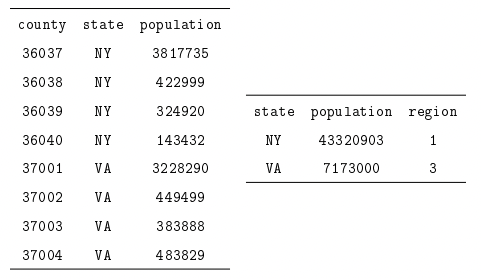
\includegraphics[width=0.6\textwidth]{normtable.png}
    \end{figure}
\end{frame}

\begin{frame}[t]{Best Practices}
    \framesubtitle{(4) Abstraction}

    \normalsize\vspace{0.5em} \begin{itemize}
        \item Abstract to eliminate redundancy \begin{itemize}
            \item If you need to perform an operation several times (e.g. computing a leave-one-out mean of variables), it is better to define a function that does it 
            \item It avoids having to copy-paste the code that computes the leave-one-out mean every time (with all the opportunities for error that that creates)
            \item Functions can also make your code more readable and clear
            \item Test your functions on fake data or small subsets of real data to verify that they work as intended
            \item Bonus: in Julia, abstracting operations into functions will greatly reduce runtime, as we saw in the previous lecture
        \end{itemize}
    \end{itemize}
\end{frame}

\begin{frame}[t]{Best Practices}
    \framesubtitle{(5) Documentation}

    \normalsize\vspace{0.5em} \begin{itemize}
        \item Write readme files and comment your code to help your future self and others understand your code \begin{itemize}
            \item Keep your documentation updated: if you change some aspect of your code, think whether the comments should also be updated. In general, avoid mentioning results / outputs in the comments as those are subject to change
        \end{itemize}
        \item Code should be self-documenting \begin{itemize}
            \item At the same time, if you write code that is clear enough, it will be clear what each piece is doing most of the time without need to comment
            \item Julia is one of the most readable languages in that sense
        \end{itemize}
    \end{itemize}
\end{frame}

\begin{frame}[t]{Additional Resources}
    \framesubtitle{Courtesy of MIT Libraries}

    \normalsize\vspace{0.5em} \begin{itemize}
        \item \href{https://docs.google.com/presentation/d/1UAtzDXer3DuLw-Wi9eAC8gwWY8XpMUAXViUCVcVupCU/edit?pli=1#slide=id.g1505c029de4_0_225}{CarpentriesMIT} is a group trying to build a local learning community for reproducible research and data skills.
              They organize occasional workshops
        \item MIT Libraries teach a series of workshops on data management. You can find more information, including resources from previous workshops, \href{https://libraries.mit.edu/data-management/services/workshops/}{here}
    \end{itemize}
\end{frame}

\section{Version Control Using Git}
\begin{frame}[t]{Basics of Git}
    \framesubtitle{What are Git and GitHub?}
    \footnotesize This section is based on guidelines from SEII and Blueprint Labs

    \normalsize\vspace{0.5em}
    \begin{itemize}
        \item Sometimes we want to keep track of changes in our code. One way to do it is to save different versions of the code, as: \texttt{Analysis\_v1.jl}, \texttt{Analysis\_v2.jl}, \texttt{Analysis\_final.jl}, \texttt{Analysis\_final\_final.jl}, \texttt{Analysis\_THE\_FINALEST.jl}
        \item Instead, consider using version control software, like Git
        \item Git allows you to track changes of text-based files over time and to access old versions. It improves your ability to work collaboratively, find and fix bugs and replicate projects
        \item By default, Git operates out of the command line. GitHub is a cloud based service that stores Git repositories on the cloud and allows users to make copies locally. It has a nice GUI called GitHub desktop that makes it even easier to use
    \end{itemize}
\end{frame}

\begin{frame}[t]{Basics of Git}
    \framesubtitle{Repositories}

    \normalsize\vspace{0.5em}
    \begin{itemize}
        \item A Git repository (repo) is a project folder that contains the code and other files that we want to track
        \item Repos can either be \alert{bare}, if they contain the history of changes but not a physical copy of the files, or \alert{non-bare}, if they contain the history of changes and a physical copy of the files
        \item A \alert{remote} repo is a bare or non-bare repository that is hosted in a location accessible to all users. It holds a common version of code history that everyone can see and access
        \item A \alert{local} repo is a non-bare repository in your personal directory. This is where you can develop code, and then send your work to the remote repo so that other team members can access it
    \end{itemize}
\end{frame}

\begin{frame}[t]{Basics of Git}
    \framesubtitle{Commits}

    \normalsize\vspace{0.5em}
    \begin{itemize}
        \item Git works by taking snapshots of your code at different points in time. Each of these snapshots is called a \alert{commit}. You decide what changes to place onto a commit; you can even save all your most recent changes while only selecting some to commit
        \item Some best practices:
        \begin{enumerate}
            \item Better to overcommit than undercommit (more tracking points), but there is a trade-off between quantity and quality
            \item Divide different types of changes into different commits (even within the same file)
            \item Accompany commits with meaningful messages, to help your future self or colleagues understand what each commit did
        \end{enumerate}
    \end{itemize}
\end{frame}

\begin{frame}[t]{Basics of Git}
    \framesubtitle{Pushing, fetching, pulling and stashing}

    \normalsize\vspace{0.5em}
    \begin{itemize}
        \item \alert{Pushing} sends the changes you committed in your local repo into the remote repo
        \item \alert{Fetching} does the reverse: it updates the local repo with any changes made at the remote
        \item \alert{Pulling} is a fetch + a merge: in addition to retrieving changes, you will merge the updated remote branch into your local version of the branch (more on branches to follow)
        \item \alert{Stashing} stores a copy of all your uncommitted changes to files and reverts the files back to their unedited state. This can be helpful if you need to switch branches temporarily but aren't ready to commit your changes yet (since you can't switch branches with uncommitted changes)
    \end{itemize}
\end{frame}

\begin{frame}[t]{Basics of Git}
    \framesubtitle{The \texttt{.gitignore} file}

    \normalsize\vspace{0.5em}
    \begin{itemize}
        \item In general, you only want to track changes in your code files, although your local repo folder will contain other files.
        \item One example of things you might want to ignore is data (for privacy/legal reasons or because they are very large files). Instead, make sure that all your collaborators have access to the raw data and track the code files that produce the clean dataset
        \item Another example is outputs: graphs, tables, pdf-ed LaTeX. PDFs, XLS and other non-ASCII files are not suitable for git. Just track the code that produces them instead, and you should be able to recover them from there
        \item The ignored files are declared in the \texttt{.gitignore} file. I'll show you how to access it in the example at the end
    \end{itemize}
\end{frame}

\begin{frame}[t]{Basics of Git}
    \framesubtitle{Issue Tracking on Github}

    \normalsize\vspace{0.5em}
    \begin{itemize}
        \item Github Issues are a very useful tool to keep track of your to-do list
        \item There are several ways to create issues and to mark them as resolved after they are addressed. The easiest is probably from the Issues tab on Github
        \item You can organize and prioritize issues with projects. To track issues as part of a larger issue, you can use task lists
        \item You can use \#labels to categorize issues, and @mention your collaborators so that they get a notification about issues
    \end{itemize}
\end{frame}

\begin{frame}[t]{Basics of Git}
    \framesubtitle{Branches}

    \normalsize\vspace{0.5em}
    \begin{itemize}
        \item \alert{Branches} have two primary uses in terms of workflow: 
        \begin{enumerate}
            \item You can work on distinct types of code edits separately by using multiple branches
            \item You can keep a \alert{master} version of the code that runs top to bottom without issues, while having a \alert{develop} branch where you work on new code
        \end{enumerate}
        \item We will talk about A Successful Git Branching Model
        \item You can incorporate changes made on one branch into another branch by \alert{merging}
    \end{itemize}
\end{frame}

\begin{frame}[t]{Basics of Git}
    \framesubtitle{Merge conflicts}

    \normalsize\vspace{0.5em}
    \begin{itemize}
        \item A merge conflict arises when there are changes made to the same line of a code file on the two branches you're trying to merge. For example, my STATA code has the line \texttt{reg Y X}. I create a branch ``robust'' where I try \texttt{reg Y X, r} instead, an another branch ``controls'' where I try \texttt{reg Y X W} instead. If I try to merge ``robust'' and ``controls,'' I will have a merge conflicts
        \item This doesn't happen if the discrepancy corresponds to different files or even different lines on the same file: the merge keeps the most recent version of those
        \item Merge conflicts need to be resolved. To do that, open the problematic file, handpick the changes that you want to keep, delete the rest, save the file and commit (this can be done on GitHub)
    \end{itemize}
\end{frame}

\begin{frame}[t]{Basics of Git}
    \framesubtitle{Merge conflicts}

    \normalsize\vspace{0.5em}
    \begin{itemize}
        \item Some best practices to avoid merge conflicts: \begin{enumerate}
            \item In your local repo, avoid working on the same section of code on two separate branches if you intend to merge them together in the future
            \item Avoid working in the same file as others on the project
            \item If you realize you've both made changes to the same file, stash your changes, pull their changes, apply your original stash, make any necessary adjustments, and push back to the origin
        \end{enumerate}
    \end{itemize}
\end{frame}

\begin{frame}[t]{A successful Git branching model}
    \framesubtitle{The main branches}
    \footnotesize This section is based on a blog post, \href{https://nvie.com/posts/a-successful-git-branching-model/}{\textit{A successful Git branching model}} by Vincent Driessen

    \normalsize\vspace{0.5em}
    \begin{columns}
        \begin{column}[t]{0.7\textwidth}
            \begin{itemize}
                \item The repository will be organized around two main branches with an infinite lifetime: \alert{master} and \alert{develop}
                \begin{itemize}
                    \item The \alert{master} branch should hold stable versions of the code that are ready to be run
                    \item The \alert{develop} branch is where those stable versions are built, and it can contain work in progress at any point in time
                    \item Once your \alert{develop} branch reaches a stable point, all changes should be merged back into \alert{master}. It is recommended to tag the merge with a version number
                \end{itemize}
            \end{itemize}    
        \end{column}
        
        \begin{column}[t]{0.25\textwidth}
            \begin{figure}
                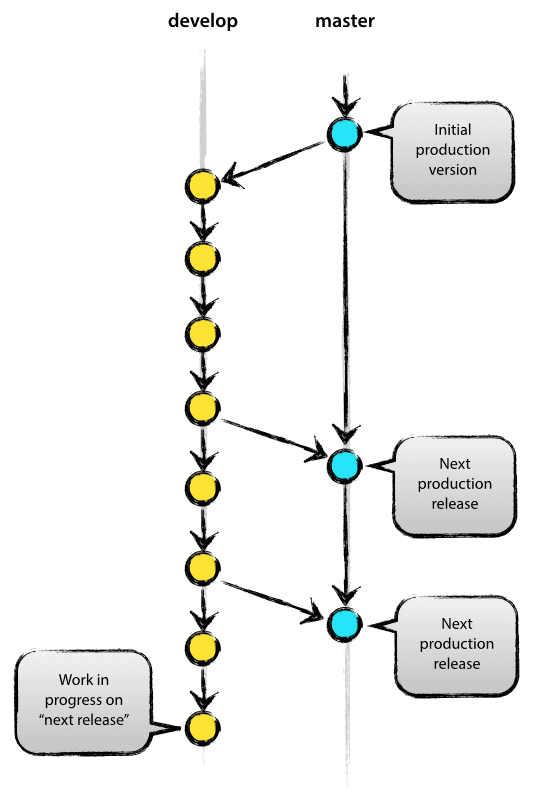
\includegraphics[width = \textwidth]{mainbr.png}
            \end{figure}
        \end{column}
    \end{columns}
\end{frame}

\begin{frame}[fragile, t]{A successful Git branching model}
    \framesubtitle{The main branches}

    \normalsize\vspace{0.5em} Here is how to merge \alert{develop} into \alert{master} from the command line:
    
    \vspace{-0.5em}
    \begin{verbatim}
            $ git checkout master
            Switched to branch 'master'
            $ git merge --no-ff develop
            Merge made by recursive.
            (Summary of changes)
            $ git tag -a 1.2    
    \end{verbatim}

    \footnotesize\vspace{-0.5em} The \texttt{--no-ff} tag causes the merge to create a new commit object so that all the commits in the merged branch before the merge are grouped together (so they can all be reverted at the same time). See the blog post for more info on this
\end{frame}

\begin{frame}[t]{A successful Git branching model}
    \framesubtitle{Supporting branches}

    \normalsize\vspace{0.5em}
    \begin{columns}
        \begin{column}[t]{0.7\textwidth}
            \begin{itemize}
                \item Supporting branches have a specific purpose and a limited life time. These can include:
                \begin{enumerate}
                    \item \alert{feature} branches. Imagine you want to try something (e.g. a different measure for the dependent variable). You can try that in a feature branch created for that purpose. These branch off from \alert{develop} and, if you're happy with it, must merge back into \alert{develop}, or otherwise, be discarded.
                    \item \alert{hotfix} branches. Imagine you discover a bug in the \alert{master} code! This needs to be fixed ASAP. You can create a specific branch for that, and merge it back into \textit{both} \alert{master} and \alert{develop}.
                \end{enumerate}
            \end{itemize}    
        \end{column}

        \begin{column}[t]{0.25\textwidth}
            \begin{figure}
                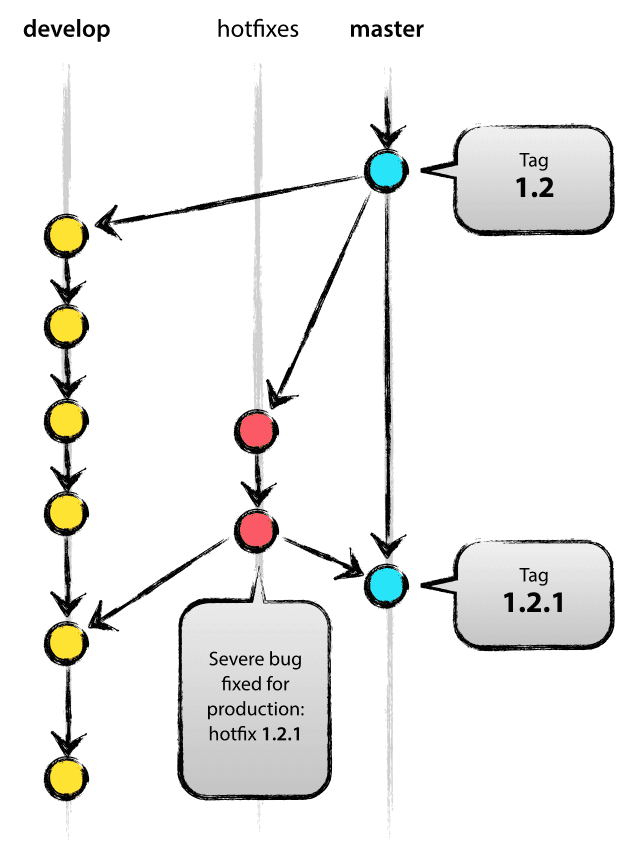
\includegraphics[width = \textwidth]{hotfixbr.png}
            \end{figure}
        \end{column}
    \end{columns}
\end{frame}

\begin{frame}[fragile, t]{A successful Git branching model}
    \framesubtitle{Supporting branches}

    \normalsize\vspace{0.5em} Here is how to create a \alert{hotfix} branch, merge to \alert{master} and \alert{develop}, and delete it from the command line:
    
    \vspace{-0.5em}
    \begin{columns}
        \begin{column}[t]{0.5\textwidth}
            \begin{verbatim}
    $ git checkout -b hotfix-1.2.1 master
    Switched to a new branch "hotfix-1.2.1"
    [...]
    $ git checkout master
    Switched to branch 'master'
    $ git merge --no-ff hotfix-1.2.1
    Merge made by recursive.
    (Summary of changes)
    $ git tag -a 1.2.1
        \end{verbatim}   
        \end{column}

        \begin{column}[t]{0.5\textwidth}
            \begin{verbatim}
    $ git checkout develop
    Switched to branch 'develop'
    $ git merge --no-ff hotfix-1.2.1
    Merge made by recursive.
    (Summary of changes)
    $ git branch -d hotfix-1.2.1
    Deleted branch hotfix-1.2.1 (was abbe5d6).
        \end{verbatim}  
        \end{column}
    \end{columns} 
\end{frame}

\begin{frame}[t]{A successful Git branching model}
    \framesubtitle{Collaborating}

    \normalsize\vspace{0.5em}
    \begin{itemize}
        \item Sometimes you will want to work in parallel with other people
        \item In that case, it may be a good idea to have a central version of the repo, called the \alert{origin}, from which every team member pulls and pushes, while every developer can have their own \alert{develop} branch locally
        \item One team member may want to pull changes from another team member's repo. This can be done with a Git remote that points to that repo
    \end{itemize}
\end{frame}
\end{document}